\documentclass[
11pt, % Set the default font size, options include: 8pt, 9pt, 10pt, 11pt, 12pt, 14pt, 17pt, 20pt
%t, % Uncomment to vertically align all slide content to the top of the slide, rather than the default centered
%aspectratio=169, % Uncomment to set the aspect ratio to a 16:9 ratio which matches the aspect ratio of 1080p and 4K screens and projectors
]{beamer}

\graphicspath{{Images/}{./}} % Specifies where to look for included images (trailing slash required)

\usepackage{todonotes}
\usepackage{graphicx}
\usepackage{xcolor}
\usepackage{subfig}
%%\usepackage[noend]{algpseudocode}

%
%\usepackage{algorithm}
%\usepackage{algorithmic}
\usepackage{algorithm}
\usepackage{algpseudocode}
\usepackage{blkarray}
\usepackage{amsmath}
\usepackage{xspace}
\usepackage{float}


\usepackage{tikz}
\usetikzlibrary{matrix, decorations, patterns, positioning, shapes, calc, intersections, arrows, fit}

\usetikzlibrary{patterns}
\usetikzlibrary{fit,calc,positioning,decorations.pathreplacing,matrix,3d, hobby}

\usepackage{booktabs} % Allows the use of \toprule, \midrule and \bottomrule for better rules in tables
\usepackage{bm}
\usepackage{multirow}
\usepackage{ragged2e}


\newcommand{\brown}[1]{{\color{brown} #1 }}

%% Colors from https://latexcolor.com/
\definecolor{pastelviolet}{rgb}{0.8, 0.6, 0.79}
\definecolor{babyblueeyes}{rgb}{0.63, 0.79, 0.95}
\definecolor{pastelyellow}{rgb}{0.99, 0.99, 0.59}
\definecolor{pastelgreen}{rgb}{0.47, 0.87, 0.47}
\definecolor{pastelred}{rgb}{1.0, 0.41, 0.38}
\colorlet{patternblue}{blue!60}

\definecolor{lightgreen}{rgb}{0, 0.5, 0}



%%\newcommand{\tensorcolor}{patternblue}
\newcommand{\tensorcolor}{cyan}


\colorlet{darkred}{red!80!black}
\colorlet{darkblue}{blue!80!black}
\newcommand<>{\darkred}[1]{{\color{darkred}{#1}}}
\newcommand<>{\darkblue}[1]{{\color#2{blue!50!black!100}{#1}}}

\newcommand{\A}{\mathbf{A}}
\newcommand{\B}{\mathbf{B}}
\newcommand{\CC}{\mathbf{C}}
%\newcommand{\Real}{\mathbb{R}}
%\newcommand{\vc}[1]{\bm{#1}}

\usetheme{Madrid}

%\newcommand{\Tra}{{\sf T}} 


%\newcommand{\Ms}[2]{\mathbf{#1}^{(#2)}} 
%\newcommand{\M}[1]{\mathbf{#1}} 
%\newcommand{\Mb}[2]{\mathbf{#1}_{#2}} 
%\newcommand{\Mbs}[3]{\mathbf{#1}_{#2}^{(#3)}} 

%\usepackage{enumitem}

\input{../tensor_header}

\newcommand{\X}{\T{X}}
\newcommand{\Y}{\T{Y}}

\newcommand{\starontop}[1]{{#1}^*}

\hypersetup{linkcolor=blue}

%----------------------------------------------------------------------------------------
%	PRESENTATION INFORMATION
%----------------------------------------------------------------------------------------

\title[Multi-TTM]{Multiple Tensor Times Matrix computation} % The short title in the optional parameter appears at the bottom of every slide, the full title in the main parameter is only on the title page

%\subtitle{Optional Subtitle} % Presentation subtitle, remove this command if a subtitle isn't required

\author[Suraj Kumar]{Suraj Kumar} % Presenter name(s), the optional parameter can contain a shortened version to appear on the bottom of every slide, while the main parameter will appear on the title slide

\institute[Inria \& ENS Lyon]{Inria \& ENS Lyon \\ \smallskip Email:\textit{suraj.kumar@ens-lyon.fr}} % Your institution, the optional parameter can be used for the institution shorthand and will appear on the bottom of every slide after author names, while the required parameter is used on the title slide and can include your email address or additional information on separate lines

\date[CR12]{CR12: October 2024\\ \smallskip\small https://surakuma.github.io/courses/daamtc.html} % Presentation date or conference/meeting name, the optional parameter can contain a shortened version to appear on the bottom of every slide, while the required parameter value is output to the title slide

%----------------------------------------------------------------------------------------

\begin{document}
	
	%----------------------------------------------------------------------------------------
	%	TITLE SLIDE
	%----------------------------------------------------------------------------------------
	
	\begin{frame}
		\titlepage % Output the title slide, automatically created using the text entered in the PRESENTATION INFORMATION block above
	\end{frame}

\begin{frame}{Tucker decomposition of $\X \in \mathbb{R}^{n_1\times n_2\times\cdots\times n_d}$}
	
	\small
	It represents a tensor with $d$ matrices (usually orthonormal) and a small core tensor.
	\vspace*{-0.25cm}\begin{center}
		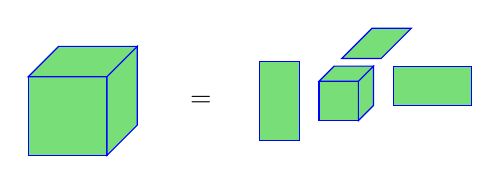
\begin{tikzpicture}[scale=0.25, every node/.style={transform shape}]
		\pgfmathsetmacro{\cubex}{4}
		\pgfmathsetmacro{\cubey}{4}
		\pgfmathsetmacro{\cubez}{4}
		\draw[blue,fill=pastelgreen] (-12,1,\cubez-2) -- ++(-\cubex,0,0) -- ++(0,-\cubey,0) -- ++(\cubex,0,0) -- cycle;
		\draw[blue,fill=pastelgreen] (-12,1,\cubez-2) -- ++(0,0,-\cubez) -- ++(0,-\cubey,0) -- ++(0,0,\cubez) -- cycle;
		\draw[blue,fill=pastelgreen] (-12,1,\cubez-2) -- ++(-\cubex,0,0) -- ++(0,0,-\cubez) -- ++(\cubex,0,0) -- cycle;
		\node[draw=none, text=black, scale=4] at (-8,-1,0) {$=$};
		
		\pgfmathsetmacro{\cubex}{2}
		\pgfmathsetmacro{\cubey}{2}
		\pgfmathsetmacro{\cubez}{2}
		\draw[blue,fill=pastelgreen] (0,0,0) -- ++(-\cubex,0,0) -- ++(0,-\cubey,0) -- ++(\cubex,0,0) -- cycle;
		\draw[blue,fill=pastelgreen] (0,0,0) -- ++(0,0,-\cubez) -- ++(0,-\cubey,0) -- ++(0,0,\cubez) -- cycle;
		\draw[blue,fill=pastelgreen] (0,0,0) -- ++(-\cubex,0,0) -- ++(0,0,-\cubez) -- ++(\cubex,0,0) -- cycle;
		
		\draw[blue,fill=pastelgreen] (-\cubex-1,1,0) -- ++(-\cubex,0,0) -- ++(0,-\cubey-2,0) -- ++(\cubex,0,0) -- cycle;
		\draw[blue,fill=pastelgreen] (\cubex+2+1,0,-\cubey) -- ++(-\cubex-2,0,0) -- ++(0,-\cubey,0) -- ++(\cubex+2,0,0) -- cycle;
		
		\draw[blue,fill=pastelgreen] (0,0,-\cubez-1) -- ++(-\cubex,0,0) -- ++(0,0,-\cubez-2) -- ++(\cubex,0,0) -- cycle;
		\end{tikzpicture}
	\end{center}
	\vspace*{-0.15cm}\centering{\footnotesize Tucker decomposition of a $3$-dimensional tensor.}
	\vfill
	{\footnotesize\vspace*{-0.1cm}$$\X = \Y \times_1 \Mn{A}{1} \cdots \times_d \Mn{A}{d}$$
		$$\X(i_1,\cdots,i_d) = \sum_{\alpha_1=1}^{r_1}\cdots\sum_{\alpha_d=1}^{r_d} \Y(\alpha_1,\cdots,\alpha_d)\Mn{A}{1}(i_1,\alpha_1)\cdots \Mn{A}{d}(i_d, \alpha_d)$$}
	\vfill
	\justifying
	It can be concisely expressed as $\X = \llbracket \Y; \Mn{A}{1}, \cdots, \Mn{A}{d}\rrbracket $.
	\vfill
	Here $r_j$ for $1\le j\le d$ denote a set of ranks. Matrices $\Mn{A}{j} \in \mathbb{R}^{n_j\times r_j}$ for $1\le j \le d$ are usually orthonormal and known as factor matrices. The tensor $\Y\in \mathbb{R}^{r_1\times r_2\times\cdots\times r_d}$ is called the core tensor. 	
\end{frame}

\begin{frame}{\large High Order SVD (HOSVD) for computing a Tucker decomposition}
	\small
	\begin{algorithm}[H]{
			\caption{HOSVD method to compute a Tucker decomposition}
			\begin{algorithmic}[1]
				\Require input tensor $\X\in \mathbb{R}^{n_1\times \cdots \times n_d}$, desired rank $(r_1,\cdots, r_d)$
				\Ensure  $\X = \Y \times_1 \Mn{A}{1} \times_2 \Mn{A}{2} \cdots \times_d \Mn{A}{d}$
				\For{$k=1 \text{ to } d$}
				\State $\Mn{A}{k}\gets r_k$ leading left singular vectors of $X_{(k)}$
				\EndFor
				\State $\Y = \X \times_1 {\Mn{A}{1}}^\Tra \times_2 {\Mn{A}{2}}^\Tra  \cdots \times_d {\Mn{A}{d}}^\Tra$
			\end{algorithmic}
	}\end{algorithm}
	
	
	\vfill
	\begin{itemize}
		\item When $r_i < rank(X_{(i)})$ for one or more $i$, the decomposition is called the truncated-HOSVD (T-HOSVD)
		\vfill
		\item The collective operation $\X \times_1 {\Mn{A}{1}}^\Tra \times_2 {\Mn{A}{2}}^\Tra  \cdots \times_d {\Mn{A}{d}}^\Tra$ is known as Multiple Tensor-Times-Matrix (Multi-TTM) computation
	\end{itemize}
\end{frame}
\begin{frame}{\large Sequentially T-HOSVD (ST-HOSVD) for Tucker decomposition}
	\small
	\begin{itemize}
		\item This method is more work efficient than T-HOSVD
		\vfill
		\item In each step, it reduces the size of one dimension of the tensor
	\end{itemize}
	
	%	\small
	\vspace{-0.25cm}\begin{algorithm}[H]{\small
			\caption{ST-HOSVD method to compute a Tucker decomposition}
			\begin{algorithmic}[1]
				\Require input tensor $\X\in \mathbb{R}^{n_1\times \cdots \times n_d}$, desired rank $(r_1,\cdots, r_d)$
				\Ensure  $\llbracket \Y; \Mn{A}{1}, \cdots, \Mn{A}{d}\rrbracket $ : a $(r_1, \cdots, r_d)$-rank Tucker decomposition of $\X$
				\State $\T{W} \gets \X$
				\For{$k=1 \text{ to } d$}
%				\State $S\gets B_{(k)}B_{(k)}^T$
				\State $\Mn{A}{k} \gets r_k$ leading singular vectors of $W_{(k)}$
				\State $\T{W} \gets \T{W} \times_k {\Mn{A}{k}}^\Tra$
				\EndFor
				\State $\Y = \T{W}$
			\end{algorithmic}
	}\end{algorithm}
%\vspace{-0.215cm}
We can note that ST-HOSVD also performs Multi-TTM computation by doing a sequence of TTM operations, i.e, $\Y =((\X \times_1 {\Mn{A}{1}}^\Tra)\times_2 {\Mn{A}{2}}^\Tra) \cdots \times_d {\Mn{A}{d}}^\Tra $.
\end{frame}

\begin{frame}{\large Bottlenecks for algorithms to compute Tucker decompositions}
	\vfill
	\begin{itemize}
		\item Multi-TTM becomes the overwhelming bottleneck computation when
		\vfill
		\begin{itemize}
			\item Matrix SVD costs are reduced using randomization via sketching or
			\vfill
			\item $\Mn{A}{k}$ are computed with eigen value decompositions of $X_{(k)}X_{(k)}^T$ (or $W_{(k)}W_{(k)}^T$)
		\end{itemize}   
	\end{itemize}
\vfill
\end{frame}
%\begin{frame}{}
%	content...
%\end{frame}



\begin{frame}{Multi-TTM computation}
	\small
	Let $\Y\in \mathbb{R}^{r_1\times\cdots\times r_d}$ be the output tensor, $\X\in \mathbb{R}^{n_1\times\cdots\times n_d}$ be the input tensor, and $\Mn{A}{k} \in \mathbb{R}^{n_k\times r_k}$ be the matrix of the $k$th mode. Then the Multi-TTM computation can be represented as 
	\vspace*{-0.25cm}$$\Y = \X \times_1 {\Mn{A}{1}}^\Tra \cdots \times_d {\Mn{A}{d}}^\Tra$$
	$$\text{ or }\X = \Y \times_1 {\Mn{A}{1}} \cdots \times_d {\Mn{A}{d}}\text.$$
	
	We will focus only on the first representation in this course. Our results and analysis extend straightforwardly to the latter case.
	
	\vfill
	\emph{Two approaches to perform this computation}:
	\begin{itemize}
		\item TTM-in-sequence approach -- performed by a sequence of TTM operations
		\vspace*{-0.15cm}$$\Y = ((\X \times_1 {\Mn{A}{1}}^\Tra)\times_2 {\Mn{A}{2}}^\Tra) \cdots \times_d {\Mn{A}{d}}^\Tra$$
	\vfill
		\item All-at-once approach
		\vspace*{-0.15cm}$$\Y(r_1^\prime,\ldots,r_d^\prime) = \sum_{\{n_k^\prime \in [n_k]\}_{k \in [d]}} \X(n_1^\prime,\ldots,n_d^\prime) \prod_{j \in [d]} \Mn{A}{j}(n_j^\prime,r_j^\prime)$$
	\end{itemize}
	\vfill
	$[d]$ denotes $\{1,2,\cdots, d\}$. We represent $n_1n_2\cdots n_d$ and $r_1r_2\cdots r_d$  by $n$ and $r$, respectively. We mainly focus on all-at-once approach.
%	 This approach reduces communication.
\end{frame}
\begin{frame}{All-at-once Multi-TTM pseudo code}
	\small
\vspace*{-0.25cm}\begin{align*}
&\text{for $n_1^\prime = 1{:}n_1$, \ldots, for $n_d^\prime = 1{:}n_d$,}\\
&\quad \text{for $r_1^\prime = 1{:}r_1$, \ldots, for $r_d^\prime = 1{:}r_d$,}\\
&\quad \quad \Y(r_1^\prime,\ldots,r_d^\prime)\  +=  \X(n_1^\prime,\ldots,n_d^\prime) \,\cdot  \Mn{A}{1}(n_{1}^\prime,r_1^\prime) \cdot \cdots \cdot \Mn{A}{N}(n_d^\prime,r_d^\prime)\\
\end{align*}
\scriptsize
\vspace*{-0.75cm}\begin{block}{$\M{\Delta}$ matrix for Multi-TTM}
	\begin{center}
		$\M{\Delta} = \begin{blockarray}{cccccccc}
		& \Mn{A}{1} & \cdots & \Mn{A}{i} & \cdots & \Mn{A}{d} & \X & \Y \\
		\begin{block}{c(ccccccc)}
		n_1^\prime & 1 & & & && 1&\\
		\vdots & & \ddots & & && \vdots&\\
		n_i^\prime & & & 1 & & & 1 &\\
		\vdots & &  & & \ddots && \vdots&\\
		n_d^\prime &  & & & & 1& 1&\\
		r_1^\prime & 1 & & & && & 1\\
		\vdots & & \ddots & & && &\vdots\\
		r_i^\prime & & & 1 & & & &1 \\
		\vdots & &  & & \ddots && & \vdots\\
		r_d^\prime &  & & & & 1& & 1\\
		\end{block}
		\end{blockarray} = \begin{pmatrix}\M{I}_{d\times d} & \V{1}_d & \V{0}_d\\ \M{I}_{d\times d} & \V{0}_d & \V{1}_d \end{pmatrix}$
	\end{center}\vspace*{-0.65cm}
\end{block}
\end{frame}

\begin{frame}{Final assignment -- deadline Oct 29}
	\vfill
\brown{Question:} Let $\Y\in \mathbb{R}^{r\times r \times r}$, $\X\in \mathbb{R}^{n \times n \times n}$ and $A \in \mathbb{R}^{n\times r}$. What are the different approaches to perform the following Multi-TTM computation?
$$\Y = \X \times_1 A^\Tra \times_2 A^\Tra \times_3 A^\Tra$$
Compute the exact number of arithmetic operations for each approach.
\vfill
\end{frame}



\section{Parallel Multi-TTM computation}
	\begin{frame}{Table of Contents}		
		\tableofcontents[currentsection,hideallsubsections] % Output the table of contents (all sections on one slide)
		\begin{block}{Settings to compute parallel communication lower bound}
			\small
			\begin{itemize}
				\item Without loss of generality, we assume that $n_1r_1\le n_2r_2\le \cdots \le n_dr_d$
				\vfill
				\item The input tensor is larger than the output tensor, i.e., $n\ge r$
				\vfill
				\item The algorithm load balances the computation -- each processor performs $1/P$th number of loop iterations
				\vfill
				\item One copy of data is in the system
				\begin{itemize}
					\item There exists a processor whose input data at the start plus output data
					at the end must be at most $\frac{n + r + \sum_{i=1}^{d}n_ir_i }{P}$ words – will analyze amount of data
					transfers for this processor
				\end{itemize}
				\vfill
				\item Assume that the innermost computation is atomic -- all the multiplications are performed on only one processor

			\end{itemize}
		\end{block}		
	\end{frame}

\subsection{$3$-dimensional Multi-TTM}
	\begin{frame}{Table of Contents}		
	\tableofcontents[currentsection,currentsubsection] % Output the table of contents (all sections on one slide)		
\end{frame}

\begin{frame}{Optimization problems (Ballard et. al., 2023)}
	\footnotesize
\vspace*{-0.25cm}\begin{lemma}
	Consider the following optimization problem:
	\vspace*{-0.15cm}$$\min_{x,y,z} x+y+z \text{ such that }$$ 
	\vspace*{-0.15cm}$$\frac{nr}{P} \le xyz, \quad
	0 \le \phantom{y}x\phantom{z} \le n_1r_1,\quad
	0 \le \phantom{x}y\phantom{z} \le n_2r_2, \quad 
	0 \le \phantom{x}z\phantom{y} \le n_3r_3,$$
%	\begin{align*}
%	\frac{nr}{P} &\le xyz  \\ 
%	,
%	\end{align*}
	where $n_1r_1 \le n_2r_2 \le n_3r_3$, and $n_1,n_2,n_3,r_1,r_2,r_3,P \ge 1$.
	The optimal solution $(\starontop{x},\starontop{y},\starontop{z})$ depends on the relative values of the constraints, yielding three cases:
	\begin{enumerate}
		\item if $P < \frac{n_3r_3}{n_2r_2}$, then $\starontop{x}=n_1r_1$, $\starontop{y}=n_2r_2$, $\starontop{z}=\frac{n_3r_3}{P}$;
		\item if $\frac{n_3r_3}{n_2r_2}\le P < \frac{n_2n_3r_2r_3}{n_1^2r_1^2}$, then $\starontop{x}=n_1r_1$, $\starontop{y}=\starontop{z}= \big(\frac{n_2n_3r_2r_3}{P}\big)^{\frac{1}{2}}$;
		\item if $\frac{n_2n_3r_2r_3}{n_1^2r_1^2} \le P$, then $\starontop{x}=\starontop{y}=\starontop{z}= \big(\frac{nr}{P}\big)^{\frac{1}{3}}$;
	\end{enumerate}
	which can be visualized as follows.
	\vspace*{-0.35cm}\begin{center}
		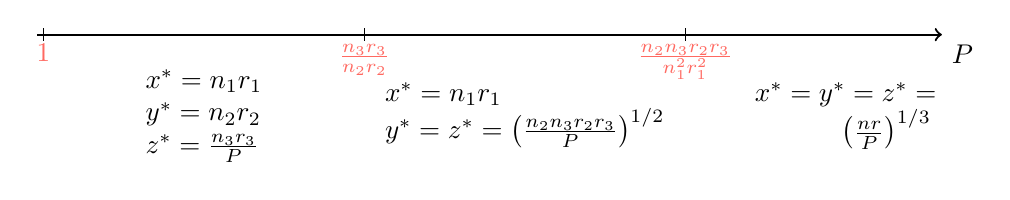
\begin{tikzpicture}[scale=0.815, every node/.style={transform shape}]
		\draw [->, thick] (-0.1,0) -- (14,0) node [below right, scale=1.2] {$P$};
		\draw (0, 0.1) -- node [below, pastelred, scale=1.2]{$1$}(0,-0.1);
		\draw (5, 0.1) -- node [below, pastelred, scale=1.2]{$\frac{n_3r_3}{n_2r_2}$}(5,-0.1);
		\draw (10, 0.1) -- node [below, pastelred, scale=1.2] {$\frac{n_2n_3r_2r_3}{n_1^2r_1^2}$}(10,-0.1);
		
		\node[align=left,below,scale=1.2] at (2.5, -0.4) {$\starontop{x}=n_1r_1$\\ $\starontop{y}=n_2r_2$\\ $\starontop{z}=\frac{n_3r_3}{P}$};
		\node[align=left,below,scale=1.2] at (7.5, -0.6) {$\starontop{x}=n_1r_1$\\$\starontop{y}=\starontop{z}= \big(\frac{n_2n_3r_2r_3}{P}\big)^{1/2}$};
		\node[align=center,below,scale=1.2] at (12.5, -0.6) {$\starontop{x}=\starontop{y}=\starontop{z}=$\\ $\qquad\quad \big(\frac{nr}{P}\big)^{1/3}$};	
		\end{tikzpicture}
	\end{center} 
\end{lemma}
\end{frame}
\begin{frame}{Optimization problems (Ballard et. al., 2023)}
	\footnotesize
	\begin{lemma}
		Consider the following optimization problem:
		\vspace*{-0.15cm}$$\min_{u,v} u+v \text{ such that }$$
		\vspace*{-0.15cm}$$\frac{nr}{P} \le uv, \quad 
		0 \le \;u\; \le r, \quad 
		0 \le \;v\; \le n,$$
		where $n\geq r$, and $n,r,P \ge 1$.
		The optimal solution $(\starontop{u},\starontop{v})$ depends on the relative values of the constraints, yielding two cases:
		\begin{enumerate}
			\item if $P < \frac{n}{r}$, then $\starontop{u}= r$, $\starontop{v} = \frac{n}{P}$;
			\item if $ \frac{n}{r} \le P$, then $\starontop{u}=\starontop{v}= \big(\frac{nr}{P}\big)^{\frac{1}{2}}$;
		\end{enumerate}
		which can be visualized as follows.
		\vspace*{-0.35cm}\begin{center}
			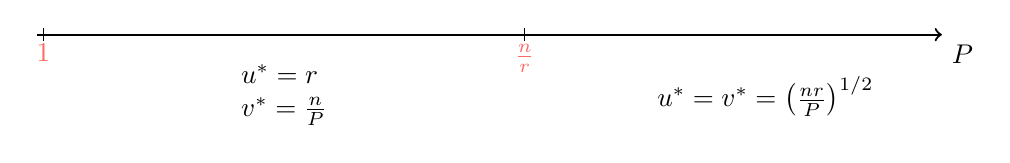
\begin{tikzpicture}[scale=0.815, every node/.style={transform shape}]
			\draw [->, thick] (-0.1,0) -- (14,0) node [below right, scale=1.2] {$P$};
			\draw (0, 0.1) -- node [below, pastelred, scale=1.2]{$1$}(0,-0.1);
			\draw (7.5, 0.1) -- node [below, pastelred, scale=1.2]{$\frac{n}{r}$}(7.5,-0.1);
			
			\node[align=left,below,scale=1.2] at (3.75, -0.325) {$\starontop{u}= r$\\ $\starontop{v} = \frac{n}{P}$};
			\node[align=left,below,scale=1.2] at (11.25, -0.5) {$\starontop{u}=\starontop{v}= \big(\frac{nr}{P}\big)^{1/2}$};
			\end{tikzpicture}
		\end{center} 
	\end{lemma}
	Both lemma can be proved using the KKT conditions.
\end{frame}

\begin{frame}{Communication lower bound}
	\small
\begin{theorem}
	Any computationally load balanced atomic Multi-TTM algorithm that starts and ends with one copy of the data distributed across processors involving 3-dimensional tensors with dimensions $n_1, n_2, n_3$ and $r_1, r_2, r_3$ performs at least $A+B-\left(\frac{n}{P}+\frac{r}{P} +\sum_{j=1}^3 \frac{n_jr_j}{P}\right)$ sends or receives where
	\begin{align*}
	A &= \begin{cases} n_1r_1 + n_2r_2 + \frac{n_3r_3}{P} & \text{ if } P<\frac{n_3r_3}{n_2r_2} \\ n_1r_1 + 2\left(\frac{n_2n_3r_2r_3}{P}\right)^{\frac{1}{2}} &\text{ if } \frac{n_3r_3}{n_2r_2}\leq P < \frac{n_2n_3r_2r_3}{n_1^2r_1^2} \\ 3\left(\frac{nr}{P}\right)^{\frac{1}{3}} &\text{ if } \frac{n_2n_3r_2r_3}{n_1^2r_1^2} \leq P\end{cases} \\
	B &= \begin{cases} r + \frac{n}{P} & \text{ if } P < \frac{n}{r} \\ 2\left(\frac{nr}{P}\right)^{\frac{1}{2}} &\text{ if } \frac{n}{r} \leq P\text.\end{cases}
	\end{align*}
\end{theorem}
\end{frame}
\begin{frame}{Communication lower bound proof}
	\small
	Let $F$ be the set of loop indices performed by a processor and $|F| = nr/P$. Define $\phi_{\X}(F)$, $\phi_{\Y}(F)$ and $\phi_j(F)$ to be the projections of $F$ onto the indices of the arrays $\X, \Y$, and $\Mn{A}{j}$ for $1\leq j\leq 3$. $\M{\Delta}$ matrix can be represented as,
		$$\M{\Delta} = \begin{pmatrix}\M{I}_{3\times 3} & \V{1}_3 & \V{0}_3\\ \M{I}_{3\times 3} & \V{0}_3 & \V{1}_3 \end{pmatrix}\text.$$ 
		$\text{Let }\mathcal{C} = \big\{\V{s} \in[0,1]^5:\M{\Delta}\cdot\V{s}\ge\V{1}\big\}\text.$
	Here $\M{\Delta}$ is not full rank, we consider all vectors $\V{v} = [a\; a\; a\; 1\text{-}a\; 1\text{-}a]^\Tra \in \mathcal{C}$ where $0\le a\le 1$ such that $\M{\Delta}\cdot\V{v}=\V{1}$. From HBL inequality, we obtain 
	{\footnotesize $$\frac{nr}{P} \leq \Big(\prod_{j\in[3]}|\phi_j(F)|\Big)^a \big(|\phi_{\X}(F)||\phi_{\Y}(F)|\big)^{1\text{-}a}\text.$$}

	This is equivalent to {\footnotesize $\frac{nr}{P} \leq \prod_{j\in[3]}|\phi_j(F)|$} and {\footnotesize $\frac{nr}{P} \leq |\phi_{\X}(F)||\phi_{\Y}(F)|$}. We also have {\footnotesize $|\phi_{\X}(F)| \leq n$}, {\footnotesize $|\phi_{\Y}(F)|\leq r$}, and {\footnotesize $|\phi_j(F)|\leq n_jr_j$} for {\footnotesize $1\leq j \leq 3$}. We want to minimize {\footnotesize $|\phi_{\X}(F)| + |\phi_{\Y}(F)| + \sum_{j\in[3]}|\phi_j(F)|$}. Employing the previous two lemmas and subtracting the owned data of the processor yields the mentioned bound. 
\end{frame}

\begin{frame}{Multi-TTM with cubical tensors}
	\small
\begin{corollary}
	\label{corollary:lb:3DMultiTTM:cubicaltensors}
	Any computationally load balanced atomic Multi-TTM algorithm that starts and ends with one copy of the data distributed across processors involving $3$-dimensional cubical tensors with dimensions $n^{\frac{1}{3}}\times n^{\frac{1}{3}}\times n^{\frac{1}{3}}$ and $r^{\frac{1}{3}}\times r^{\frac{1}{3}}\times r^{\frac{1}{3}}$ (with $n\geq r$) performs at least
	$$3\left(\frac{nr}{P}\right)^{\frac{1}{3}} + r - \frac{3(nr)^{\frac{1}{3}}+r}{P}$$
	sends or receives when $P<\frac{n}{r}$ and at least
	$$3\left(\frac{nr}{P}\right)^{\frac{1}{3}}+2\left(\frac{nr}{P}\right)^{\frac{1}{2}} - \frac{n+3(nr)^{\frac{1}{3}}+r}{P}$$
	sends or receives when $P \geq \frac{n}{r}$.
\end{corollary}

\vfill
We will manily focus on $P<\frac{n}{r}$ case throughout the slides.
\end{frame}
\begin{frame}{Data distribution model}
	\small
	$P$ processors are organized in a $6$-dimensional $p_1 \times p_2 \times p_3 \times q_1 \times q_2 \times q_3$ logical processor grid.
	\vfill
	\begin{center}
			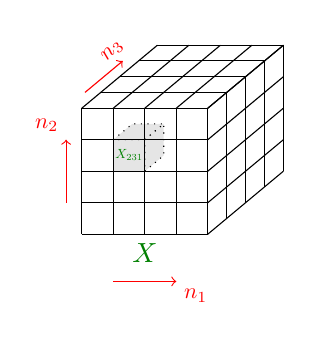
\begin{tikzpicture}[scale=0.4, every node/.style={transform shape}]
		\def\xref{0.6}
		\def\yref{0.5}
		
		\draw [dotted,fill=gray!20] (-1,2) -- (0,2) -- (0,3) --(-1,3) --(-1,2);
		\draw [dotted,fill=gray!20] (-1, 3) -- (-1+\xref,3+\yref) -- (0+\xref,3+\yref) -- (0,3) -- (-1, 3) ;
		\draw [dotted,fill=gray!20] (0, 2) -- (0+\xref,2+\yref) -- (0+\xref,3+\yref) -- (0,3) -- (0,2);
		
		
		\foreach \y in {0, 1, 2, 3, 4}
		\draw (-2, \y) -- (2, \y);
		
		\foreach \x in {-2, -1, 0, 1, 2}
		\draw (\x, 0) -- (\x, 4);
		
		\foreach \y in {0, 1, 2, 3, 4}
		\draw (2, \y)--(2+4*\xref, 4*\yref+\y);
		
		
		\foreach \y in {0, 1, 2, 3, 4}
		\draw (2+\y * \xref, \y * \yref) -- (2+\y * \xref, 4+\y * \yref);
		
		\foreach \x in {-2, -1, 0, 1, 2}
		\draw (\x, 4) -- (\x + 4*\xref, 4+4*\yref);
		
		\foreach \y in {0, 1, 2, 3, 4}
		\draw (-2+\y * \xref, 4+\y * \yref) -- (2+\y * \xref, 4+\y * \yref);
		
		\node [below, lightgreen, scale=2.5] at (0,0) {$\T{X}$};
		
		%%	\draw [dotted] (-1, 3) -- (-1+\xref,3+\yref);
		%%	\draw [dotted] (0, 3) -- (0+\xref,3+\yref);
		%%	\draw [dotted] (0, 2) -- (0+\xref,2+\yref);
		%%	\draw [dotted] (-1+\xref,3+\yref) -- (0+\xref,3+\yref);
		%%	\draw [dotted] (0+\xref,3+\yref) -- (0+\xref,2+\yref);
		
		
		\node [ lightgreen, scale=1.2] at (-0.5,2.5) {$\T{X}_{231}$};
		
		\draw [->, red] (-1,-1.5) -- (1,-1.5) node [below right, scale=2] {$n_1$};
		\draw [->, red] (-2.5,1) -- (-2.5,3) node [ above left, scale=2] {$n_2$};
		\draw [->, red] (-2.5+\xref, 4+\yref) -- (-2.5 + 3*\xref, 4+3*\yref) node [above,rotate=45, scale=2] {$n_3$};
		\end{tikzpicture}$\qquad$
		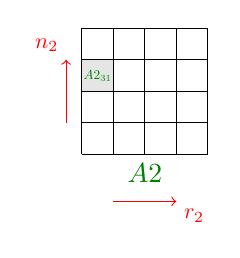
\begin{tikzpicture}[scale=0.4, every node/.style={transform shape}]
		\def\xref{0.6}
		\def\yref{0.5}
		\draw [fill=gray!20] (-2,2) -- (-1,2) -- (-1,3) --(-2,3) --(-2,2);
		
		\foreach \y in {0, 1, 2, 3, 4}
		\draw (-2, \y) -- (2, \y);
		
		\foreach \x in {-2, -1, 0, 1, 2}
		\draw (\x, 0) -- (\x, 4);
		
		\node [below, lightgreen, scale=2.5] at (0,0) {$\Mn{A}{2}$};
		
		
		\node [ lightgreen, scale=1.2] at (-1.5,2.5) {$\Mn{A}{2}_{31}$};
		
		\draw [->, red] (-1,-1.5) -- (1,-1.5) node [below right, scale=2] {$r_2$};
		\draw [->, red] (-2.5,1) -- (-2.5,3) node [ above left, scale=2] {$n_2$};
		\end{tikzpicture}
	\end{center}
Subtensor $\T{X}_{231}$ is distributed evenly among processors $(2,3,1,*,*,*)$. Similarly, submatrix $\Mn{A}{2}_{31}$ is distributed evenly among processors $(*,3,*,*,1,*)$.
\end{frame}
\begin{frame}{Parallel Multi-TTM algorithm}
	
\begin{algorithm}[H]\small
	\caption{Parallel Atomic 3-dimensional Multi-TTM}
	\begin{algorithmic}[1]
		\Require $\T{X}$, $\Mn{A}{1}$, $\Mn{A}{2}$, $\Mn{A}{3}$, $p_1 \times p_2 \times p_3 \times q_1 \times q_2 \times q_3$ logical processor grid
		\Ensure $\T{Y}$ such that $\Y = \X \times_1 {\Mn{A}{1}}^\Tra \times_2 {\Mn{A}{2}}^\Tra \times_3 {\Mn{A}{3}}^\Tra$
		\State $(p_1^\prime, p_2^\prime, p_3^\prime, q_1^\prime, q_2^\prime, q_3^\prime)$ is my processor id
		\State //All-gather input tensor $\T{X}$
		\State $\T{X}_{p_1^\prime p_2^\prime p_3^\prime}$ = All-Gather($\T{X}$, $(p_1^\prime, p_2^\prime, p_3^\prime, *, *, *)$)
		\State //All-gather input matrices
		\State $\Mn{A}{1}_{p_1^\prime q_1^\prime}$ = All-Gather($\Mn{A}{1}$, $(p_1^\prime, *, *, q_1^\prime, *, *)$)
		\State $\Mn{A}{2}_{p_2^\prime q_2^\prime}$ = All-Gather($\Mn{A}{2}$, $(*, p_2^\prime, *, *, q_2^\prime, *)$)
		\State $\Mn{A}{3}_{p_3^\prime q_3^\prime}$ = All-Gather($\Mn{A}{3}$, $(*, *, p_3^\prime, *, *, q_3^\prime)$)
		\State //Local computations in a temporary tensor $\T{T}$
		\State $\T{T}$ = Local-Multi-TTM($\T{X}_{p_1^\prime p_2^\prime p_3^\prime}$, $\Mn{A}{1}_{p_1^\prime q_1^\prime}$, $\Mn{A}{2}_{p_2^\prime q_2^\prime}$, $\Mn{A}{3}_{p_3^\prime q_3^\prime}$)
		\State //Reduce-scatter the output tensor in $\T{Y}_{q_1^\prime q_2^\prime q_3^\prime}$
		\State Reduce-Scatter($\T{Y}_{q_1^\prime q_2^\prime q_3^\prime}$, $\T{T}$, $(*, *, *, q_1^\prime, q_2^\prime, q_3^\prime)$)\label{alg:3dmultittm:line:reduceScatterOutputTensor}
	\end{algorithmic}
\end{algorithm}
\end{frame}

\begin{frame}{Steps of the algorithm}
	\small
\begin{figure}
	\begin{center}
		\subfloat[{\scriptsize Perform All-Gather on processors $(2,1,1,*,*,*)$ to obtain $\T{X}_{211}$.}]{
			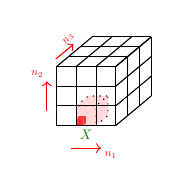
\begin{tikzpicture}[scale=0.25, every node/.style={transform shape}]
			\def\xref{0.6}
			\def\yref{0.5}
			
			\draw [dotted,fill=red!15] (1,0) -- (2,0) -- (2,1) --(1,1) --(1,0);
			\draw [dotted,fill=red!15] (1,1) --(1+\xref, 1+\yref) -- (2+\xref,1+\yref) -- (2,1) -- (1,1);
			\draw [dotted,fill=red!15] (2,0) -- (2+\xref, 0+\yref) -- (2+\xref, 1+\yref) -- (2,1) -- (2,0);
			
			\def\a{1}
			\def\b{0}
			\def\xstride{0.35}
			\def\ystride{0.35}
			\draw [draw=none,fill=red!80] (\a,\b) -- (\a+\xstride,\b) -- (\a+\xstride,\b+\ystride) --(\a,\b+\ystride) --(\a,\b);
			
			\def\xsmallref{0.135}
			\def\ysmallref{0.125}
			\draw [draw=none,fill=red!80] (\a,\b+\ystride) --(\a+\xsmallref, \b+\ystride+\ysmallref) -- (\a+\xstride+\xsmallref, \b+\ystride+\ysmallref) -- (\a+\xstride, \b+\ystride) -- (\a, \b+\ystride);
			
			\draw [draw=none,fill=red!80] (\a+\xstride,\b) --(\a+\xstride+\xsmallref, \b+\ysmallref) -- (\a+\xstride+\xsmallref, \b+\ystride+\ysmallref) -- (\a+\xstride, \b+\ystride) -- (\a+\xstride, \b);
			
			\foreach \y in {0, 1, 2, 3}
			\draw (0, \y) -- (3, \y);
			
			\foreach \x in {0, 1, 2, 3}
			\draw (\x, 0) -- (\x, 3);
			
			\foreach \y in {0, 1, 2, 3}
			\draw (3, \y)--(3+3*\xref, 3*\yref+\y);
			
			
			\foreach \y in {0, 1, 2, 3}
			\draw (3+\y * \xref, \y * \yref) -- (3+\y * \xref, 3+\y * \yref);
			
			\foreach \x in {0, 1, 2, 3}
			\draw (\x, 3) -- (\x + 3*\xref, 3+3*\yref);
			
			\foreach \y in {0, 1, 2, 3}
			\draw (0+\y * \xref, 3+\y * \yref) -- (3+\y * \xref, 3+\y * \yref);
			
			\node [below, lightgreen, scale=2] at (1.5,0) {$\T{X}$};
			
			
			\draw [->, red] (0.75,-1.15) -- (2.25,-1.15) node [below right, scale=1.6] {$n_1$};
			\draw [->, red] (-0.5,0.75) -- (-0.5,2.25) node [ above left, scale=1.6] {$n_2$};
			\draw [->, red] (-0.5+0.75*\xref, 3+0.75*\yref) -- (-0.5 + 2.25*\xref, 3+2.25*\yref) node [above,rotate=45, scale=1.6] {$n_3$};
			\path (0,0) -- (4.75,0);
			\end{tikzpicture}}$\ $
		\subfloat[{\scriptsize Perform All-Gather on processors $(2,*,*,1,*,*)$ to obtain $\Mn{A}{1}_{21}$.}]{
			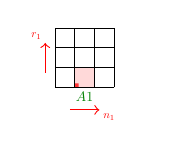
\begin{tikzpicture}[scale=0.25, every node/.style={transform shape}]
			
			\draw [dotted,fill=red!15] (1,0) -- (2,0) -- (2,1) --(1,1) --(1,0);
			
			\def\a{1}
			\def\b{0}
			\def\xstride{0.2}
			\def\ystride{0.2}
			\draw [draw=none,fill=red!80] (\a,\b) -- (\a+\xstride,\b) -- (\a+\xstride,\b+\ystride) --(\a,\b+\ystride) --(\a,\b);
			
			\foreach \y in {0, 1, 2, 3}
			\draw (0, \y) -- (3, \y);
			
			\foreach \x in {0, 1, 2, 3}
			\draw (\x, 0) -- (\x, 3);
			
			\node [below, lightgreen, scale=2] at (1.5,0) {$\Mn{A}{1}$};
			
			\draw [->, red] (0.75,-1.15) -- (2.25,-1.15) node [below right, scale=1.6] {$n_1$};
			\draw [->, red] (-0.5,0.75) -- (-0.5,2.25) node [ above left, scale=1.6] {$r_1$};
			\path (0,0) -- (4.75,0);
			\end{tikzpicture}}$\ $
		\subfloat[{\scriptsize Perform All-Gather on processors $(*,1,*,*,3,*)$ to obtain $\Mn{A}{2}_{13}$.}]{
			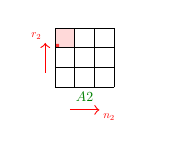
\begin{tikzpicture}[scale=0.25, every node/.style={transform shape}]
			
			\draw [dotted,fill=red!15] (0,2) -- (1,2) -- (1,3) --(0,3) --(0,2);
			
			\def\a{0}
			\def\b{2}
			\def\xstride{0.2}
			\def\ystride{0.2}
			\draw [draw=none,fill=red!80] (\a,\b) -- (\a+\xstride,\b) -- (\a+\xstride,\b+\ystride) --(\a,\b+\ystride) --(\a,\b);
			
			\foreach \y in {0, 1, 2, 3}
			\draw (0, \y) -- (3, \y);
			
			\foreach \x in {0, 1, 2, 3}
			\draw (\x, 0) -- (\x, 3);
			
			\node [below, lightgreen, scale=2] at (1.5,0) {$\Mn{A}{2}$};
			
			\draw [->, red] (0.75,-1.15) -- (2.25,-1.15) node [below right, scale=1.6] {$n_2$};
			\draw [->, red] (-0.5,0.75) -- (-0.5,2.25) node [ above left, scale=1.6] {$r_2$};
			\path (0,0) -- (4.75,0);
			\end{tikzpicture}}$\ $
		\subfloat[{\scriptsize Perform All-Gather on processors $(*,*,1,*,*,1)$ to obtain $\Mn{A}{3}_{11}$.}]{
			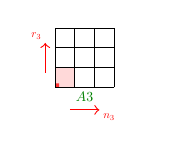
\begin{tikzpicture}[scale=0.25, every node/.style={transform shape}]
			
			\draw [dotted,fill=red!15] (0,0) -- (1,0) -- (1,1) --(0,1) --(0,0);
			
			\def\a{0}
			\def\b{0}
			\def\xstride{0.2}
			\def\ystride{0.2}
			\draw [draw=none,fill=red!80] (\a,\b) -- (\a+\xstride,\b) -- (\a+\xstride,\b+\ystride) --(\a,\b+\ystride) --(\a,\b);
			
			\foreach \y in {0, 1, 2, 3}
			\draw (0, \y) -- (3, \y);
			
			\foreach \x in {0, 1, 2, 3}
			\draw (\x, 0) -- (\x, 3);
			
			\node [below, lightgreen, scale=2] at (1.5,0) {$\Mn{A}{3}$};
			
			\draw [->, red] (0.75,-1.15) -- (2.25,-1.15) node [below right, scale=1.6] {$n_3$};
			\draw [->, red] (-0.5,0.75) -- (-0.5,2.25) node [ above left, scale=1.6] {$r_3$};
			\path (0,0) -- (4.75,0);
			\end{tikzpicture}}$\ $
		\subfloat[{\scriptsize Perform local Multi-TTM to compute partial $\T{Y}_{131}$.\label{fig:step:partialResults}}]{
			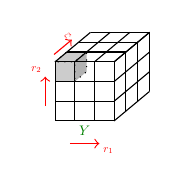
\begin{tikzpicture}[scale=0.25, every node/.style={transform shape}]
			\def\xref{0.6}
			\def\yref{0.5}
			\draw [dotted,fill=gray!40] (0,2) -- (1,2) -- (1,3) --(0,3) --(0,2);
			\draw [dotted,fill=gray!40] (0,3) --(0+\xref, 3+\yref) -- (1+\xref,3+\yref) -- (1,3) -- (0,3);
			\draw [dotted,fill=gray!60] (1,2) -- (1+\xref, 2+\yref) -- (1+\xref, 3+\yref) -- (1,3) -- (1,2);
			
			\foreach \y in {0, 1, 2, 3}
			\draw (0, \y) -- (3, \y);
			
			\foreach \x in {0, 1, 2, 3}
			\draw (\x, 0) -- (\x, 3);
			
			\foreach \y in {0, 1, 2, 3}
			\draw (3, \y)--(3+3*\xref, 3*\yref+\y);
			
			\foreach \y in {0, 1, 2, 3}
			\draw (3+\y * \xref, \y * \yref) -- (3+\y * \xref, 3+\y * \yref);
			
			\foreach \x in {0, 1, 2, 3}
			\draw (\x, 3) -- (\x + 3*\xref, 3+3*\yref);
			
			\foreach \y in {0, 1, 2, 3}
			\draw (0+\y * \xref, 3+\y * \yref) -- (3+\y * \xref, 3+\y * \yref);
			
			\node [below, lightgreen, scale=2] at (1.5,0) {$\T{Y}$};
			
			\draw [->, red] (0.75,-1.15) -- (2.25,-1.15) node [below right, scale=1.6] {$r_1$};
			\draw [->, red] (-0.5,0.75) -- (-0.5,2.25) node [ above left, scale=1.6] {$r_2$};
			\draw [->, red] (-0.5+0.75*\xref, 3+0.75*\yref) -- (-0.5 + 2.25*\xref, 3+2.25*\yref) node [above,rotate=45, scale=1.2] {$r_3$};
			\path (0,0) -- (4.75,0);
			\end{tikzpicture}}$\ $
		\subfloat[{\scriptsize Perform Reduce-Scatter on processors $(*,*,*,1,3,1)$ to compute/distribute $\T{Y}_{131}$.}]{
			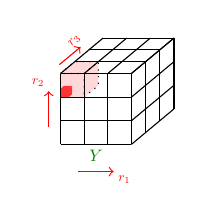
\begin{tikzpicture}[scale=0.3, every node/.style={transform shape}]
			\def\xref{0.6}
			\def\yref{0.5}
			\draw [dotted,fill=red!15] (0,2) -- (1,2) -- (1,3) --(0,3) --(0,2);
			\draw [dotted,fill=red!15] (0,3) --(0+\xref, 3+\yref) -- (1+\xref,3+\yref) -- (1,3) -- (0,3);
			\draw [dotted,fill=red!15] (1,2) -- (1+\xref, 2+\yref) -- (1+\xref, 3+\yref) -- (1,3) -- (1,2);
			
			
			
			\def\a{0}
			\def\b{2}
			\def\xstride{0.35}
			\def\ystride{0.35}
			\draw [draw=none,fill=red!80] (\a,\b) -- (\a+\xstride,\b) -- (\a+\xstride,\b+\ystride) --(\a,\b+\ystride) --(\a,\b);
			
			\def\xsmallref{0.135}
			\def\ysmallref{0.125}
			\draw [draw=none,fill=red!80] (\a,\b+\ystride) --(\a+\xsmallref, \b+\ystride+\ysmallref) -- (\a+\xstride+\xsmallref, \b+\ystride+\ysmallref) -- (\a+\xstride, \b+\ystride) -- (\a, \b+\ystride);
			
			\draw [draw=none,fill=red!80] (\a+\xstride,\b) --(\a+\xstride+\xsmallref, \b+\ysmallref) -- (\a+\xstride+\xsmallref, \b+\ystride+\ysmallref) -- (\a+\xstride, \b+\ystride) -- (\a+\xstride, \b);
			
			
			\foreach \y in {0, 1, 2, 3}
			\draw (0, \y) -- (3, \y);
			
			\foreach \x in {0, 1, 2, 3}
			\draw (\x, 0) -- (\x, 3);
			
			\foreach \y in {0, 1, 2, 3}
			\draw (3, \y)--(3+3*\xref, 3*\yref+\y);
			
			\foreach \y in {0, 1, 2, 3}
			\draw (3+\y * \xref, \y * \yref) -- (3+\y * \xref, 3+\y * \yref);
			
			\foreach \x in {0, 1, 2, 3}
			\draw (\x, 3) -- (\x + 3*\xref, 3+3*\yref);
			
			\foreach \y in {0, 1, 2, 3}
			\draw (0+\y * \xref, 3+\y * \yref) -- (3+\y * \xref, 3+\y * \yref);
			
			\node [below, lightgreen, scale=2] at (1.5,0) {$\T{Y}$};
			
			\draw [->, red] (0.75,-1.15) -- (2.25,-1.15) node [below right, scale=1.6] {$r_1$};
			\draw [->, red] (-0.5,0.75) -- (-0.5,2.25) node [ above left, scale=1.6] {$r_2$};
			\draw [->, red] (-0.5+0.75*\xref, 3+0.75*\yref) -- (-0.5 + 2.25*\xref, 3+2.25*\yref) node [above,rotate=45, scale=1.6] {$r_3$};
			\path (0,0) -- (4.925,0);
			\end{tikzpicture}}
%		\caption{Hello}
%		\caption{}
	\end{center}	
\end{figure}
Steps of the algorithm for processor $(2,1,1,1,3,1)$, where $p_1=p_2=p_3=q_1=$\linebreak$q_2=q_3=3$. Highlighted areas correspond to the data blocks on which the processor is operating. The dark red highlighting represents the input/output data initially/finally owned by the processor, and the light red highlighting corresponds to received/sent data from/to other processors in All-Gather/Reduce-Scatter collectives to compute $\T{Y}_{131}$.	
\end{frame}
\begin{frame}{Cost analysis}
	\small
The bandwidth cost of the algorithm is 
$$\frac{n}{p} + \frac{n_1r_1}{p_1q_1} + \frac{n_2r_2}{p_2q_2} + \frac{n_3r_3}{p_3q_3} + \frac{r}{q} - \left(\frac{n + n_1r_1 + n_2r_2 + n_3r_3 + r}{P}\right)\text.$$
Here $p=p_1p_2p_3$ and $q=q_1q_2q_3$. The algorithm is communication optimal when we select $p_i$ and $q_i$ based on lower bounds.
\begin{block}{Arithmetic operations}
The dimensions of $\T{X}_{p_1^\prime p_2^\prime p_3^\prime}$ and $\T{T}$ are $\frac{n_1}{p_1} \times \frac{n_2}{p_2} \times \frac{n_3}{p_3}$ and $\frac{r_1}{q_1} \times \frac{r_2}{q_2} \times \frac{r_3}{q_3}$, respectively. The dimension of  $\Mn{A}{k}_{p_k^\prime q_k^\prime}$ is $\frac{n_i}{p_i}\times \frac{r_i}{q_i}$ for $i=1,2,3$.
\begin{itemize}
	\item Local Multi-TTM can be performed as a sequence of TTM operations
	\item Assuming TTM operations are performed in their order, first with $\Mn{A}{1}$, then with $\Mn{A}{2}$, and in the end with $\Mn{A}{3}$,
	$$\text{ Total arithmetic operations } = 2\Big(\frac{n_1n_2n_3r_1}{p_1p_2p_3q_1} + \frac{n_2n_3r_1r_2}{p_2p_3q_1q_2} + \frac{n_3r_1r_2r_3}{p_3q_1q_2q_3}\Big)\text.$$
\end{itemize}
\end{block}
\end{frame}
\begin{frame}{Multi-TTM cost in TuckerMPI library}
	\small
	\begin{itemize}
		\item State-of-the-art library for parallel Tucker decomposition
		\item Implements ST-HOSVD algorithm -- employs TTM-in-sequence approach to perform Multi-TTM
		\item Assume TTMs are performed in increasing mode order 
	\end{itemize}
It uses a $\tilde{p_1}\times \tilde{p_2}\times \tilde{p_3}$ logical processor grid. The bandwidth cost is
\begin{align*}
\frac{r_1n_2n_3}{\tilde{p_2}\tilde{p_3}} + \frac{n_1r_1}{\tilde{p_1}} + \frac{r_1r_2n_3}{\tilde{p_1}\tilde{p_3}} +\frac{n_2r_2}{\tilde{p_2}} + \frac{r_1r_2r_3}{\tilde{p_1}\tilde{p_2}} + \frac{n_3r_3}{\tilde{p_3}} \phantom{\frac{r_1r_2n_3}{\tilde{p_1}\tilde{p_3}}}\qquad\qquad \\ \phantom{\frac{r_1r_2n_3}{\tilde{p_1}\tilde{p_3}}}\qquad\qquad - \frac{r_1n_2n_3+r_1r_2n_3+r_1r_2r_3 + n_1r_1 +n_2r_2+n_3r_3}{P}\text. \notag
\end{align*}
The parallel computational cost is 
$$2 \left( \frac{r_1n_1n_2n_3+r_1r_2n_2n_3+r_1r_2r_3n_3}{P}\right)\text.$$
\end{frame}
\begin{frame}{Comparison of All-at-once and TTM-in-sequence}
	\small
\begin{figure}
	\begin{center}
%		\includegraphics[scale=0.195]{./legend-comm-comp.png}
%		\includegraphics[scale=0.195]{./all-at-once-seq-label.png}
		\includegraphics[scale=0.135]{./course-label.png}
	\end{center}\setcounter{subfigure}{0}
	\vspace*{-0.575cm}\begin{center}
		\subfloat[$n_i=2^{8}$, $r_i=2^{3}$.]{\includegraphics[width=0.32\linewidth]{./A@O-vs-Seq-logscale-comparison-with-comp-8-8-8-3-3-3.eps}}\hfill
		\subfloat[$n_i=2^{11}$, $r_i=2^{5}$.]{\includegraphics[width=0.32\linewidth]{./A@O-vs-Seq-logscale-comparison-with-comp-11-11-11-5-5-5.eps}}\hfill
		\subfloat[$n_i=2^{15}$, $r_i=2^{6}$.]{	\includegraphics[width=0.32\linewidth]{./A@O-vs-Seq-logscale-comparison-with-comp-15-15-15-6-6-6.eps}}
	\end{center}
\end{figure}
		\only<1>{Communication cost comparison of all-at-once approach (the presented algorithm) and TTM-in-sequence approach (of TuckerMPI). $Comp$-$Overhead$ shows the percentage of computational overhead of the all-at-once approach with respect to the TTM-in-sequence approach. Cost of an approach represents the minimum cost among all possible processor configurations.}
		\only<2>{
		\begin{itemize}
			\item Not any clear winner for all settings
			\item All-at-once approach performs significantly less communication for small $P$ 
			\item Computational overhead of all-at-once approach is negligible for small $P$
			\item TTM-in-sequence approach is better for large $P$
		\end{itemize}
		}
\end{frame}

\subsection{$d$-dimensional Multi-TTM}
\begin{frame}{Table of Contents}		
	\tableofcontents[currentsection,currentsubsection] % Output the table of contents (all sections on one slide)		
\end{frame}
\begin{frame}{Communication lower bound}
	\small
\begin{theorem}
	Any computationally load balanced atomic Multi-TTM algorithm that starts and ends with one copy of the data distributed across processors and involves $d$-dimensional tensors with dimensions $n_1, n_2, \ldots, n_d$ and $r_1, r_2, \ldots, r_d$ performs at least $A+B-\left(\frac{n}{P}+\frac{r}{P} +\sum_{j=1}^d \frac{n_jr_j}{P}\right)$ sends or receives where
	\begin{align*}
	A &= \begin{cases} \sum_{j=1}^{d\text{-}1}n_jr_j + \frac{N_1R_1}{P} &\text{ if } P<\frac{N_1R_1}{n_{d\text{-}1}r_{d\text{-}1}}\text,\\
	\sum_{j=1}^{(d\text{-}i)} n_jr_j + i\left(\frac{N_{i}R_{i}}{P}\right)^\frac{1}{i} &\text{ if } \frac{N_{i\text{-}1}R_{i\text{-}1}}{(n_{d+1\text{-}i}r_{d+1\text{-}i})^{i\text{-}1}} \leq P < \frac{N_{i}R_{i}}{(n_{d\text{-}i}r_{d\text{-}i})^i}\text, \\
	& \hfill \text{for some } 2\leq i\leq d-1, \\
	d\left(\frac{N_dR_d}{P}\right)^\frac{1}{d} &\text{ if } \frac{N_{d\text{-}1}R_{d\text{-}1}}{(n_1r_1)^{d\text{-}1}} \leq P\text.
	\end{cases}\\
	B &= \begin{cases} r + \frac{n}{P} & \text{ if } P < \frac{n}{r}\text, \\ 2\left(\frac{nr}{P}\right)^{\frac{1}{2}} &\text{ if } \frac{n}{r} \leq P\text.\end{cases}
	\end{align*}
\end{theorem}
\end{frame}
\begin{frame}{Parallel Multi-TTM algorithm}
	\small
\vspace*{-0.25cm}\begin{algorithm}[H]\small
	\caption{\label{alg:genMultittm}Parallel Atomic d-dimensional Multi-TTM}
	\begin{algorithmic}[1]
		\Require $\T{X}$, $\Mn{A}{1}$, $\cdots$, $\Mn{A}{d}$, $p_1 \times \cdots \times p_d \times q_1 \times \cdots \times q_d$ logical processor grid
		\Ensure $\T{Y}$ such that $\Y = \X \times_1 {\Mn{A}{1}}^\Tra \cdots \times_d {\Mn{A}{d}}^\Tra$
		\State $(p_1^\prime, \cdots , p_d^\prime, q_1^\prime, \cdots, q_d^\prime)$ is my processor id
		\State //All-gather input tensor $\T{X}$
		\State $\T{X}_{p_1^\prime \cdots p_d^\prime}$ = All-Gather($\T{X}$, $(p_1^\prime, \cdots , p_d^\prime, *, \cdots, *)$)\label{alg:genMultittm:line:allGatherInputTensor}
		\State //All-gather all input matrices
		\For{$i=1,\cdots, d$} 
		\State $\Mn{A}{i}_{p_i^\prime q_i^\prime}$ = All-Gather($\Mn{A}{i}$, $(*,\cdots,*, p_i^\prime,* \cdots,*, q_i^\prime, *)$)\label{alg:genMultittm:line:allGatherMatrixi} 
		\EndFor
		\State //Perform local computations in a temporary tensor $\T{T}$
		\State $\T{T}$ = Local-Multi-TTM($\T{X}_{p_1^\prime \cdots p_d^\prime}$, $\Mn{A}{1}_{p_1^\prime q_1^\prime}$,$\cdots$, $\Mn{A}{d}_{p_d^\prime q_d^\prime}$)\label{alg:genMultittm:line:localcomputation}
		\State //Reduce-scatter the output tensor in $\T{Y}_{q_1^\prime \cdots q_d^\prime}$
		\State Reduce-Scatter($\T{Y}_{q_1^\prime \cdots q_d^\prime}$, $\T{T}$, $(*, \cdots , *, q_1^\prime, \cdots, q_d^\prime)$)\label{alg:genMultittm:line:reduceScatterOutputTensor}
	\end{algorithmic}
\end{algorithm}
The algorithm is communication optimal when $p_i$ and $q_i$ are selected based on the lower bound.
\vfill
\end{frame}
\begin{frame}{Perspectives}
	\small
	\begin{itemize}
		\item Cost analysis of several ways to perform Multi-TTM
		\begin{itemize}
			\item Unifying all-at-once and sequence approaches
			%			\vfill
			\item Study of communication-computation trade-off
		\end{itemize}
		\vfill
		\item Optimal costs for algorithms to compute Tucker decompositions
		\vfil
		\item Design and implementation of parallel optimal algorithms
	\end{itemize}
\end{frame}
\end{document} 